\section{Cross-Episodic Curriculum: Formalism and Implementations}
\label{sec:method}
In this section, we establish the foundation for our cross-episodic curriculum method by first reviewing the preliminaries underlying our case studies, which encompass two representative scenarios in sequential decision-making. Subsequently, we formally introduce the assembly of curricular data and the specifics of model optimization utilizing cross-episodic attention. Lastly, we delve into the practical implementation of \cec in the context of these two scenarios.

\subsection{Preliminaries}
\para{Reinforcement learning.}
We consider the setting where source agents learn through trial and error in partially observable environments.
Denoting states $s \in \mathcal{S}$ and actions $a \in \mathcal{A}$, an agent interacts in a Partially Observable Markov Decision Process (POMDP) with the transition function $p(s_{t + 1} \vert s_t, a_t): \mathcal{S} \times \mathcal{A} \rightarrow \mathcal{S}$. It observes $o \in \mathcal{O}$ emitted from observation function $\Omega(o_t \vert s_t, a_{t - 1}): \mathcal{S} \times \mathcal{A} \rightarrow \mathcal{O}$ and receives scalar reward $r$ from $R (s, a): \mathcal{S} \times \mathcal{A} \rightarrow \mathbb{R}$.
Under the episodic task setting,
RL seeks to learn a parameterized policy $\pi_\theta (\cdot \vert s)$ that maximizes the return over a fixed length $T$ of interaction steps: $\pi_\theta = \arg \max_{\theta \in \Theta} \sum_{t = 0}^{T - 1} \gamma^t r_t$, where $\gamma \in [0, 1)$ is a discount factor.
Here we follow the canonical definition of an episode $\tau$ as a series of environment-agent interactions with length $T$, $\tau \vcentcolon= (s_0, a_0, r_0, \ldots, s_{T - 1}, a_{T - 1}, r_{T - 1}, s_T)$, where initial states $s_0$ are sampled from initial state distribution $s_0 \sim \rho_0(s)$ and terminal states $s_T$ are reached once the elapsed timestep exceeds $T$.
Additionally, we view all RL tasks considered in this work as goal-reaching problems~\citep{Kaelbling1993LearningTA,ghosh2019learning} and constrain all episodes to terminate upon task completion.
It is worth noting that similar to previous work~\citep{laskin2023incontext}, training data are collected by source RL agents during their online learning. Nevertheless, once the dataset is obtained, our method is trained \emph{offline} in a purely supervised manner.

\para{Imitation learning.}
We consider IL settings with existing trajectories composed only of state-action pairs.
Furthermore, we relax the assumption on demonstration optimality and allow them to be crowdsourced~\citep{brown2019extrapolating,chen2020learning,cao2021learning}.
Data collected by operators with varying expertise are therefore unavoidable. 
Formally, we assume the access to a dataset $\mathcal{D}^N \vcentcolon= \{\tau_1, \ldots, \tau_{N}\}$ consisting of $N$ demonstrations, with each demonstrated trajectory $\tau_i \vcentcolon= (s_0, a_0, \ldots, s_{T - 1}, a_{T - 1})$ naturally identified as an episode.
The goal of IL, specifically of behavior cloning (BC), is to learn a policy $\pi_\theta$ that accurately models the distribution of behaviors.
When viewed as goal-reaching problems, BC policies can be evaluated by measuring the success ratio in completing tasks~\citep{ghosh2019learning}.

\subsection{Curricular Data Assembly and Model Optimization}
Meaningful learning signals emerge when multiple trajectories are organized and examined cross-episodically along a curriculum axis.
This valuable information, which is not easily discernible in individual training episodes, may encompass aspects such as the improvement of an RL agent's navigation policy or the generally effective manipulation skills exhibited by operators with diverse proficiency levels.
With a powerful model architecture such as Transformer~\cite {vaswani2017attention,dai2019transformerxl}, such emergent and valuable learning signals can be baked into policy weights, thereby boosting performance in embodied tasks.

For a given embodied task $\mathcal{M}$, we define its curriculum $\mathcal{C}_\mathcal{M}$ as a collection of trajectories $\tau$ consisting of state-action pairs.
A series of ordered levels $[\mathcal{L}_1, \ldots, \mathcal{L}_L]$ partitions this collection such that $\bigcup_{l \in \{1, \ldots, L\}} \mathcal{L}_{l} = \mathcal{C}_\mathcal{M}$ and $\bigcap_{\forall i, j \in \{1, \ldots, L\}, i \neq j} \mathcal{L}_{\{i, j\}} = \emptyset$.
More importantly, these ordered levels characterize a curriculum by encoding, for example, learning progress in single environments, learning progress in a series of progressively harder environments, or the increase of the demonstrator's expertise.

With a curriculum $\mathcal{C}_\mathcal{M} \vcentcolon= \{\tau_i\}_{i = 1}^N$ and its characteristics $[\mathcal{L}_1, \ldots, \mathcal{L}_L]$, we construct a curricular sequence $\mathcal{T}$ that spans multiple episodes and captures the essence of gradual improvement in the following way:
\begin{equation}
    \mathcal{T} \vcentcolon= \bigoplus_{l \in \{1, \ldots, L\}} \left[\tau^{(1)}, \ldots, \tau^{(C)} \right], \quad  \text{where} \quad C \sim  \mathcal{U}\left(\llbracket \vert \mathcal{L}_l \vert \rrbracket\right) \quad \text{and} \quad \tau^{(c)} \sim \mathcal{L}_l.
\end{equation}
The symbol $\oplus$ denotes the concatenation operation. $\mathcal{U}\left( \llbracket K \rrbracket \right)$ denotes a uniform distribution over the discrete set $\{k \in \mathbb{N}, k\leq K \}$. In practice, we use values smaller than $\vert \mathcal{L}_l \vert$ considering the memory consumption.

We subsequently learn a causal policy that only depends on cross-episodic historical observations $\pi_\theta (\cdot \vert o_{\leq t}^{(\leq n)})$.
Note that this modeling strategy differs from previous work that views sequential decision-making as a big sequence-modeling problem~\citep{chen2021decisiontransformer,janner2021onebigsequence,laskin2023incontext,jiang2022vima}. It instead resembles the causal policy in \citet{openai2022vpt}. Nevertheless, we still follow the best practice~\citep{for-the-win,openai2019dota,fan2022minedojo} to provide previous action as an extra modality of observations in POMDP RL tasks.

We leverage the powerful attention mechanism of Transformer~\citep{vaswani2017attention} to enable cross-episodic attention.
Given observation series $O_t^{(n)} \vcentcolon= \{o_{0}^{(1)},\ldots, o_{\leq t}^{(\leq n)} \}$ (shorthanded as $O$ hereafter for brevity), 
Transformer projects it into query $Q = f_Q(O)$, key $K = f_K (O)$, and value $V = f_V(O)$ matrices, with each row being a $D$-dim vector.
Attention operation is performed to aggregate information:
\begin{equation}
    \text{Attention}(Q, K, V) = \text{softmax}(\frac{QK^\intercal}{\sqrt{D}})V.
\end{equation}
Depending on whether the input arguments for $f_Q$ and $f_{\{K, V\}}$ are the same, attention operation can be further divided into self-attention and cross-attention.
Since tasks considered in this work do not require additional conditioning for task specification, 
we follow previous work~\citep{openai2022vpt,zhu2022viola} to utilize self-attention to process observation series.
Nevertheless, ours can be naturally extended to handle, for example, natural language or multi-modal task prompts, following the cross-attention introduced in \citet{jiang2022vima}.

Finally, this Transformer policy is trained by simply minimizing the negative log-likelihood objective $\mathcal{J}_{\text{NLL}}$ of labeled actions, conditioned on cross-episodic context:
\begin{equation}
    \mathcal{J}_{\text{NLL}} =   - \log \pi_\theta (\cdot \vert \mathcal{T}) = \frac{1}{\vert \mathcal{T} \vert \times T} \sum_{n = 1}^{\vert \mathcal{T} \vert} \sum_{t = 1}^T - \log \pi_\theta \left(a_t^{(n)} \vert  o_{\leq t}^{(\leq n)} \right).
\end{equation}
Regarding the specific memory architecture, we follow \citet{openai2022vpt,team2023humantimescale} to use Transformer-XL~\citep{dai2019transformerxl} as our model backbone. Thus, during deployment, we keep its hidden states propagating across test episodes to mimic the training settings.

\subsection{Practical Implementations}
We now discuss concrete instantiations of \cec for 1) RL with DMLab and 2) IL with RoboMimic.
Detailed introductions to the benchmark and task selection are deferred to Sec.~\ref{sec:exp_setup}.
We investigate the following three curricula, where the initial two pertain to RL, while the final one applies to IL:

\para{Learning-progress-based curriculum.}
In the first instantiation, inspired by the literature on learning progress~\citep{matiisen2017teacherstudent,graves2017automated,portelas2019teacher,kanitscheider2021multitask}, we view the progression of learning agents as a curriculum.
Concretely, we train multi-task PPO agents~\citep{schulman2017proximal,petrenko2020sample} on tasks drawn from test distributions.
We record their online interactions during training, which faithfully reflect the learning progress.
Finally, we form the \textit{learning-progress-based curriculum} by sequentially concatenating episodes collected at different learning stages.
Note that this procedure is different from \citet{laskin2023incontext}, where for each environment, the learning dynamics of \emph{multiple} single-task RL agents has to be logged. In contrast, we only track a \emph{single} multi-task agent per environment.
\begin{figure}[t]
    \centering
    \begin{subfigure}[t]{0.19\textwidth}
        \centering
        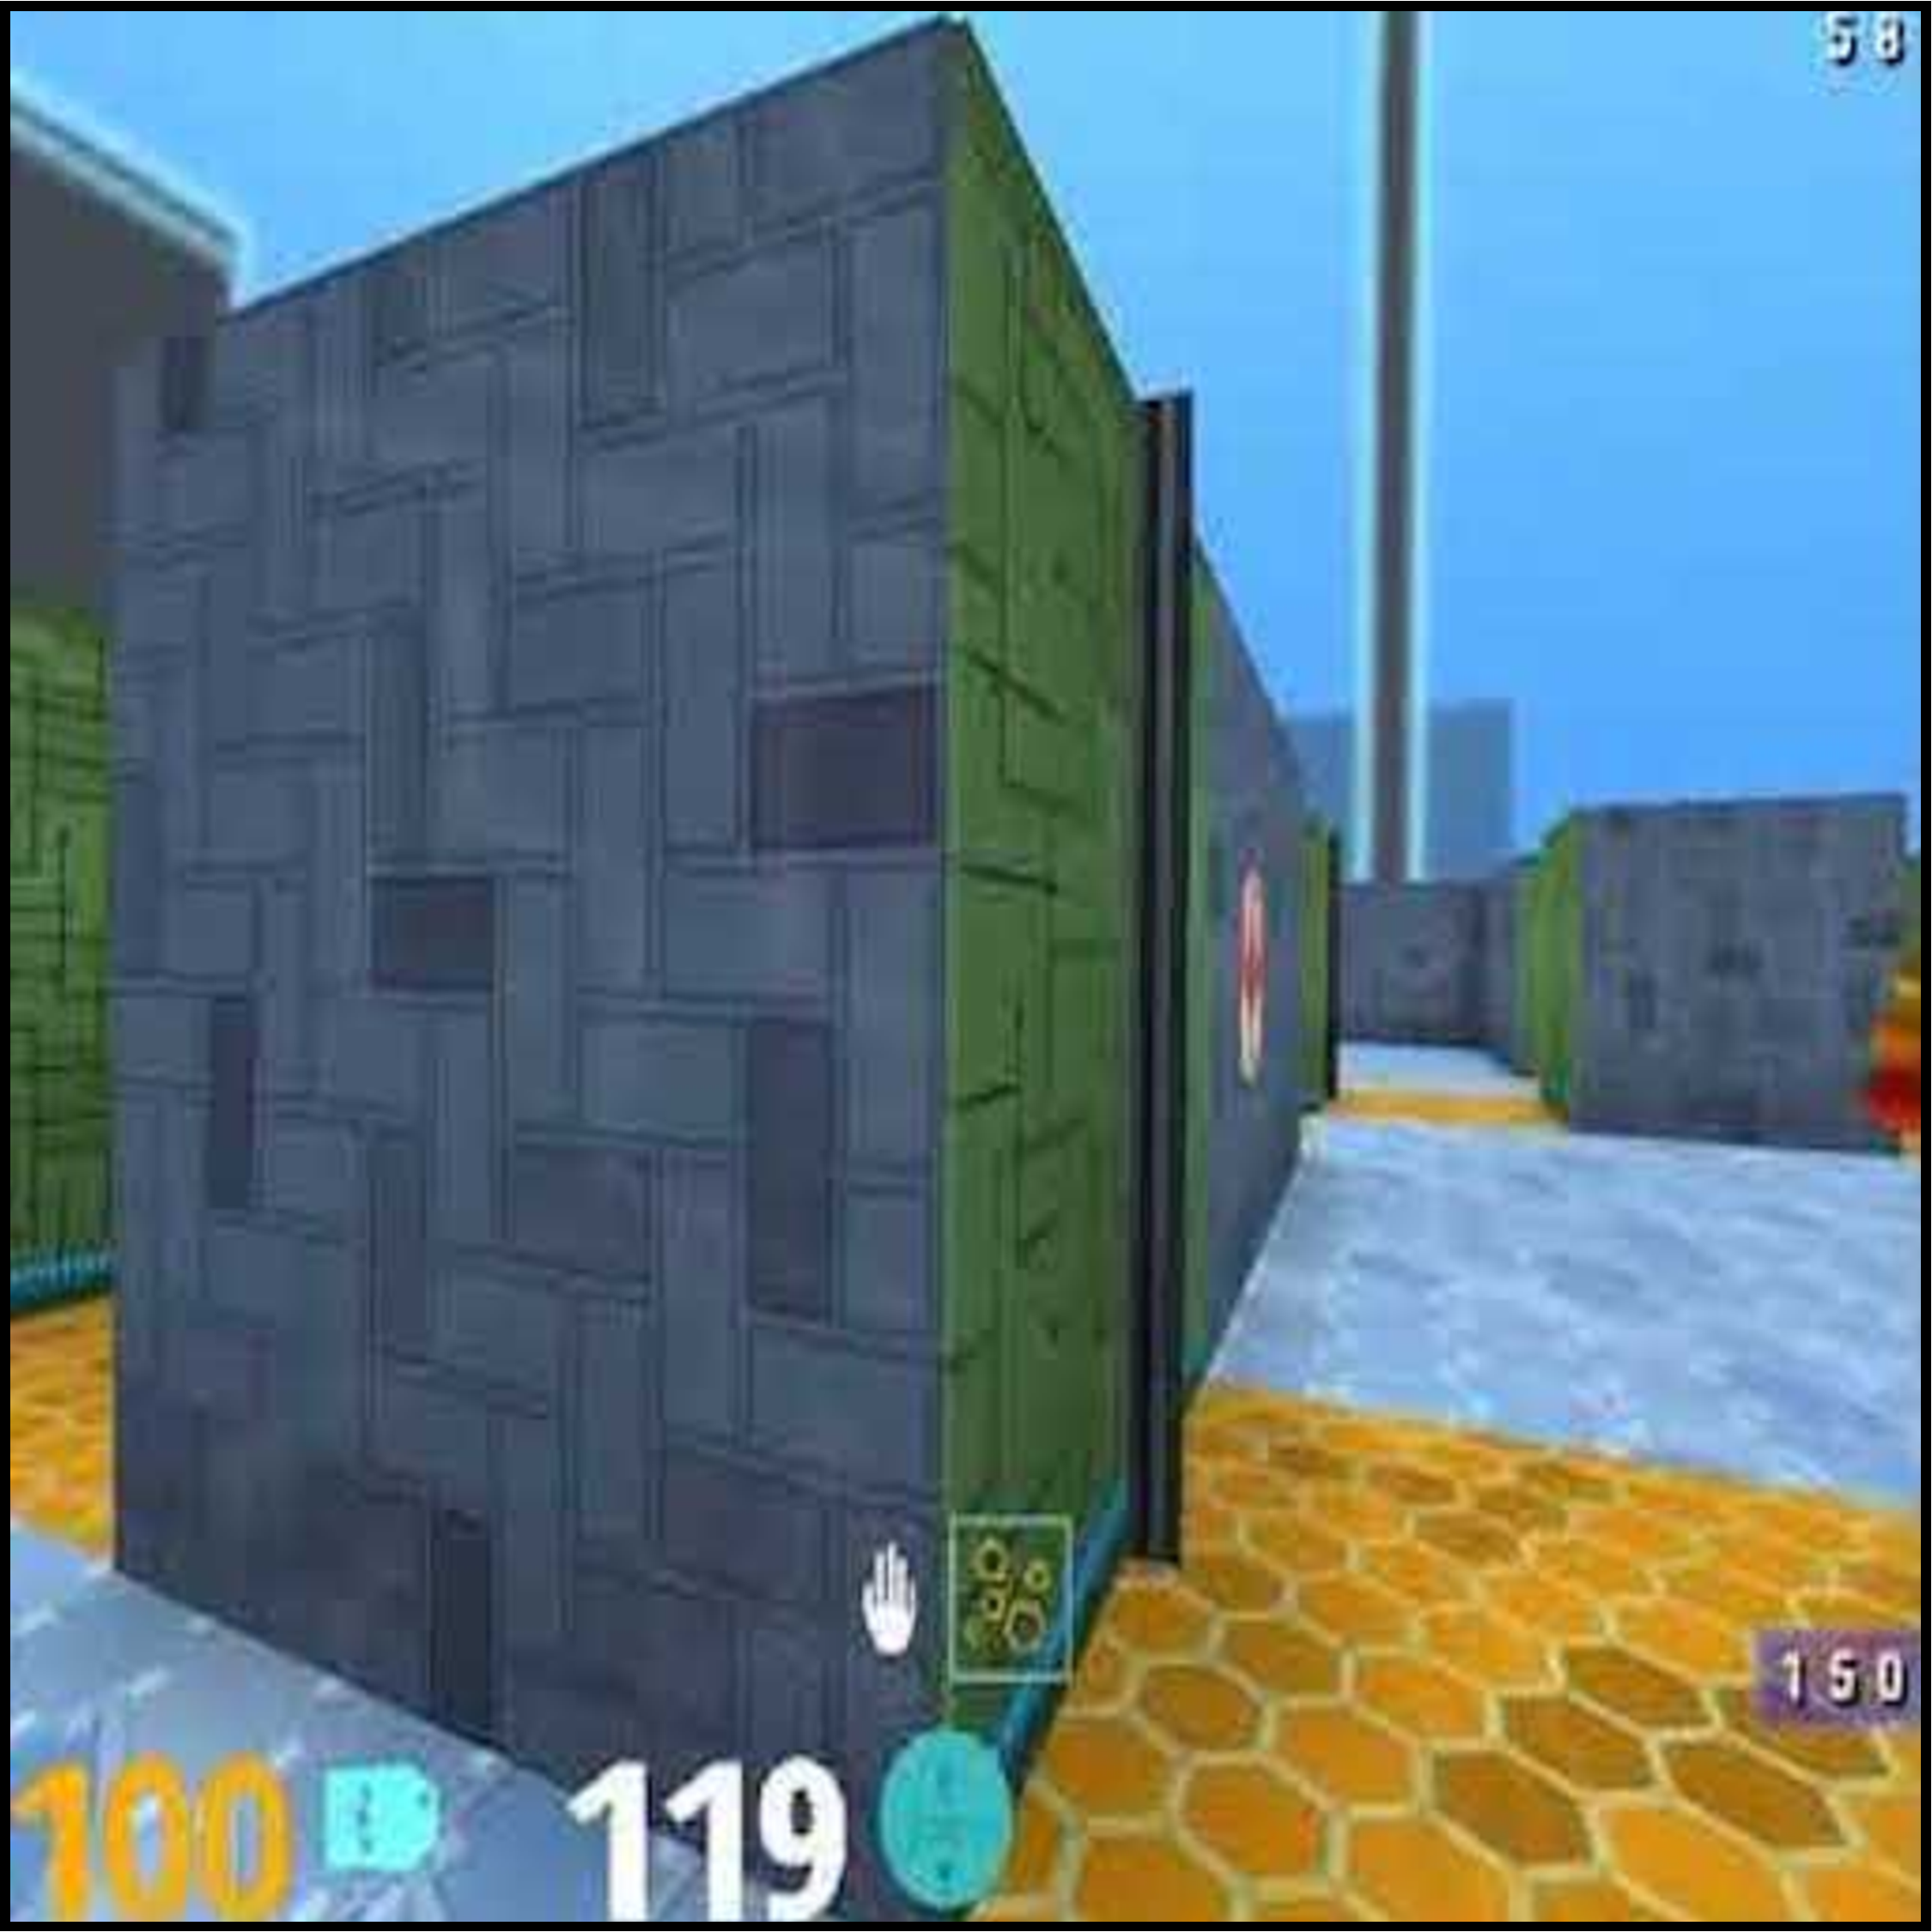
\includegraphics[width=\textwidth]{fig/tasks/goal_maze.pdf}
        \caption{Goal Maze}
        \label{fig:tasks:goal_maze}
    \end{subfigure} 
    \hfill
    \begin{subfigure}[t]{0.19\textwidth}
        \centering
        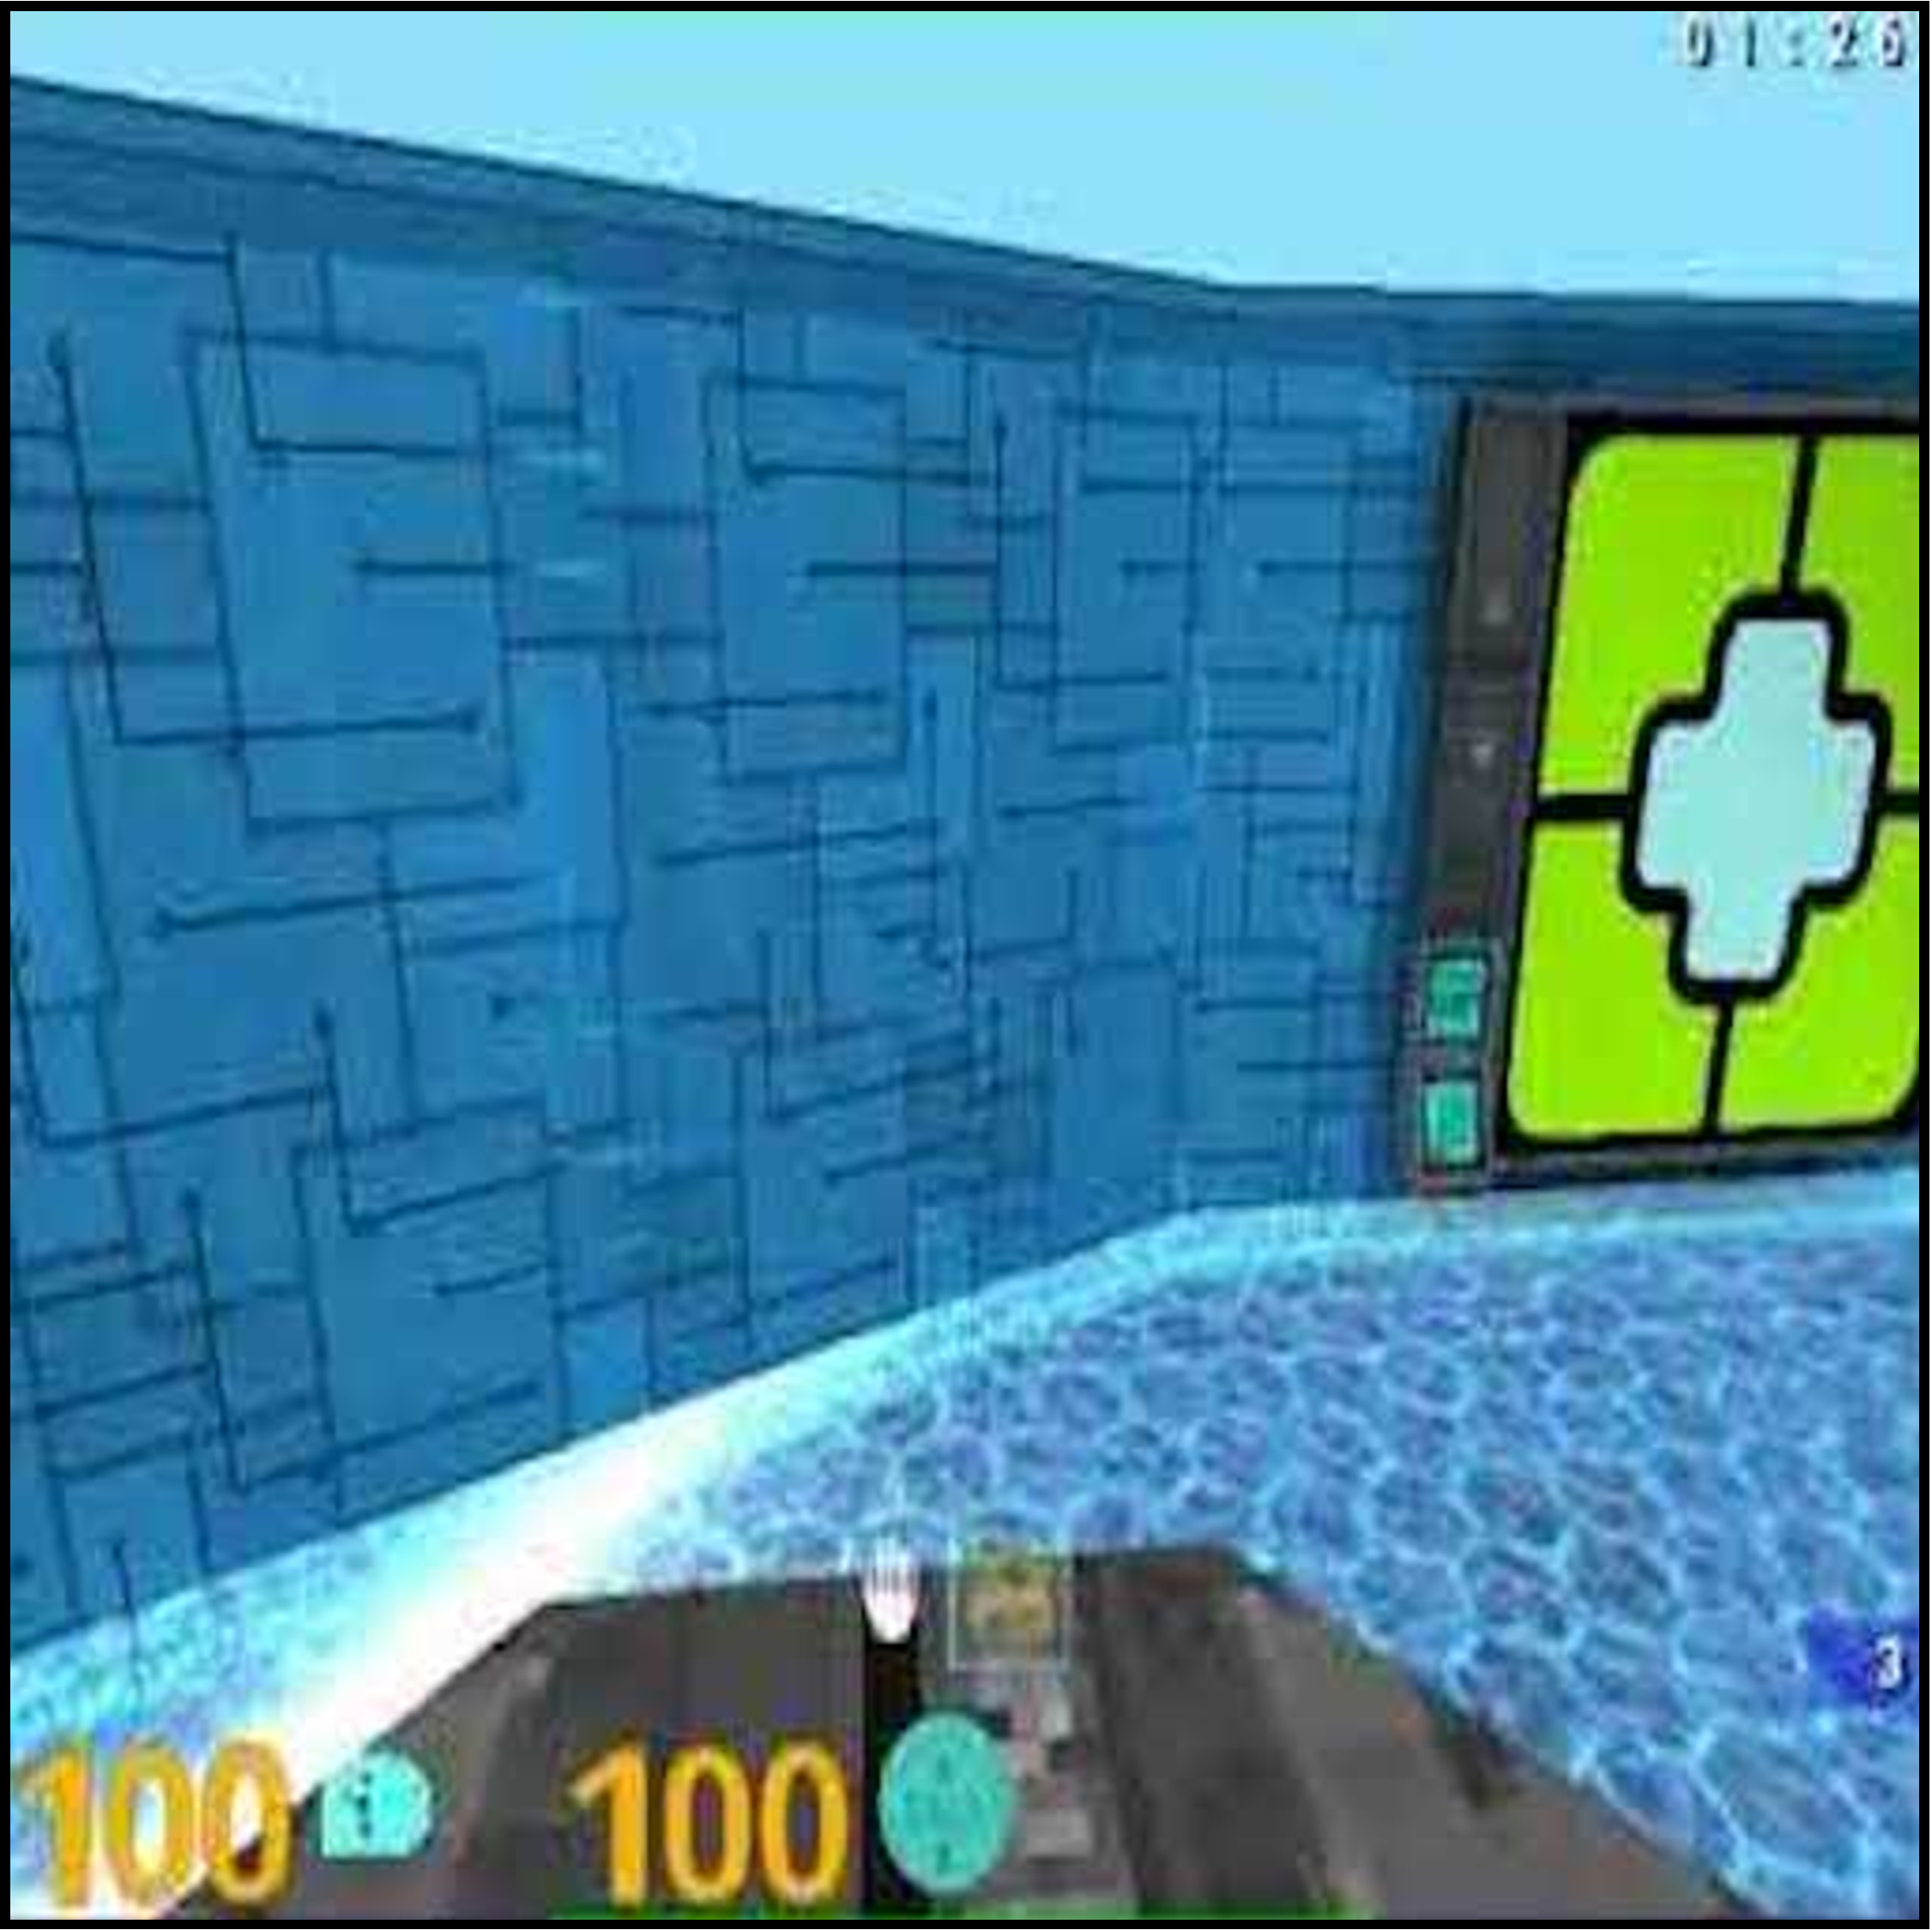
\includegraphics[width=\textwidth]{fig/tasks/watermaze.pdf}
        \caption{Watermaze}
        \label{fig:tasks:watermaze}
    \end{subfigure}
    \hfill
    \begin{subfigure}[t]{0.19\linewidth}
        \centering
        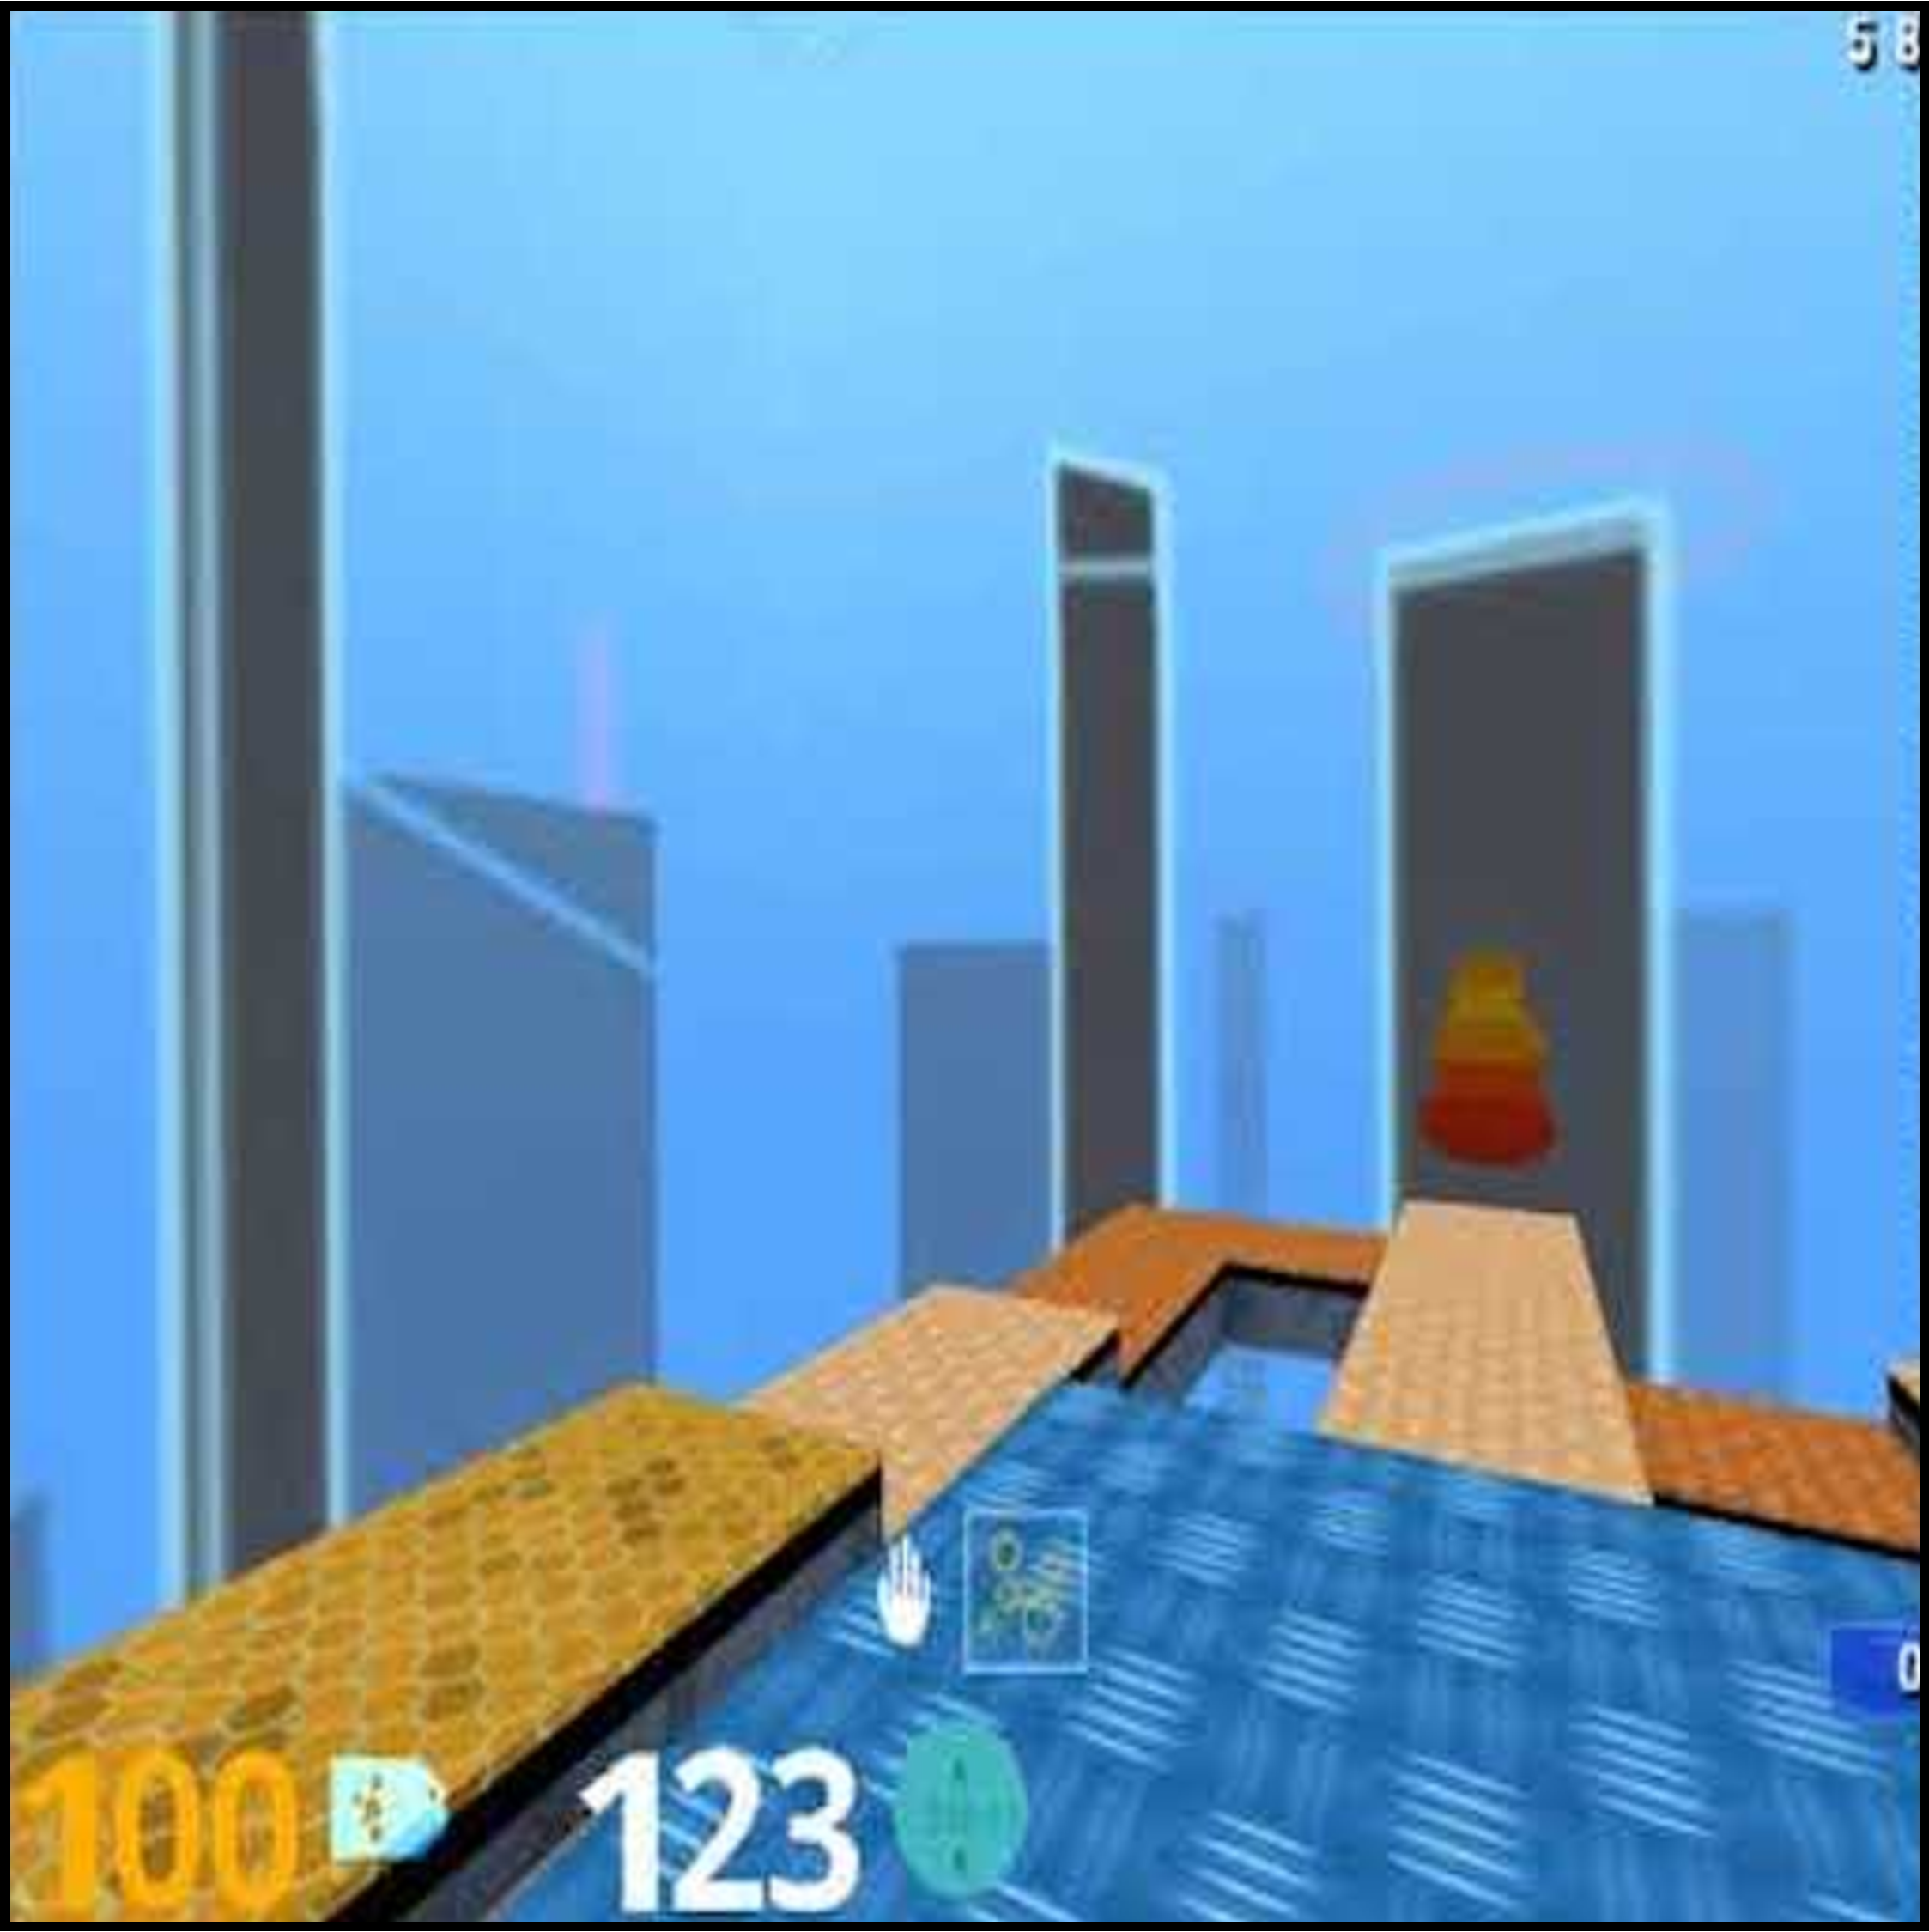
\includegraphics[width=\linewidth]{fig/tasks/irreversible_path.pdf}
        \caption{Irreversible Path}
        \label{fig:tasks:irreversible_path}
    \end{subfigure}
    \hfill
    \begin{subfigure}[t]{0.19\linewidth}
        \centering
        
\includegraphics[width=\linewidth]{fig/tasks/lift.pdf}
        \caption{Lift}
        \label{fig:tasks:lift}
    \end{subfigure} 
    \hfill
    \begin{subfigure}[t]{0.19\linewidth}
        \centering
        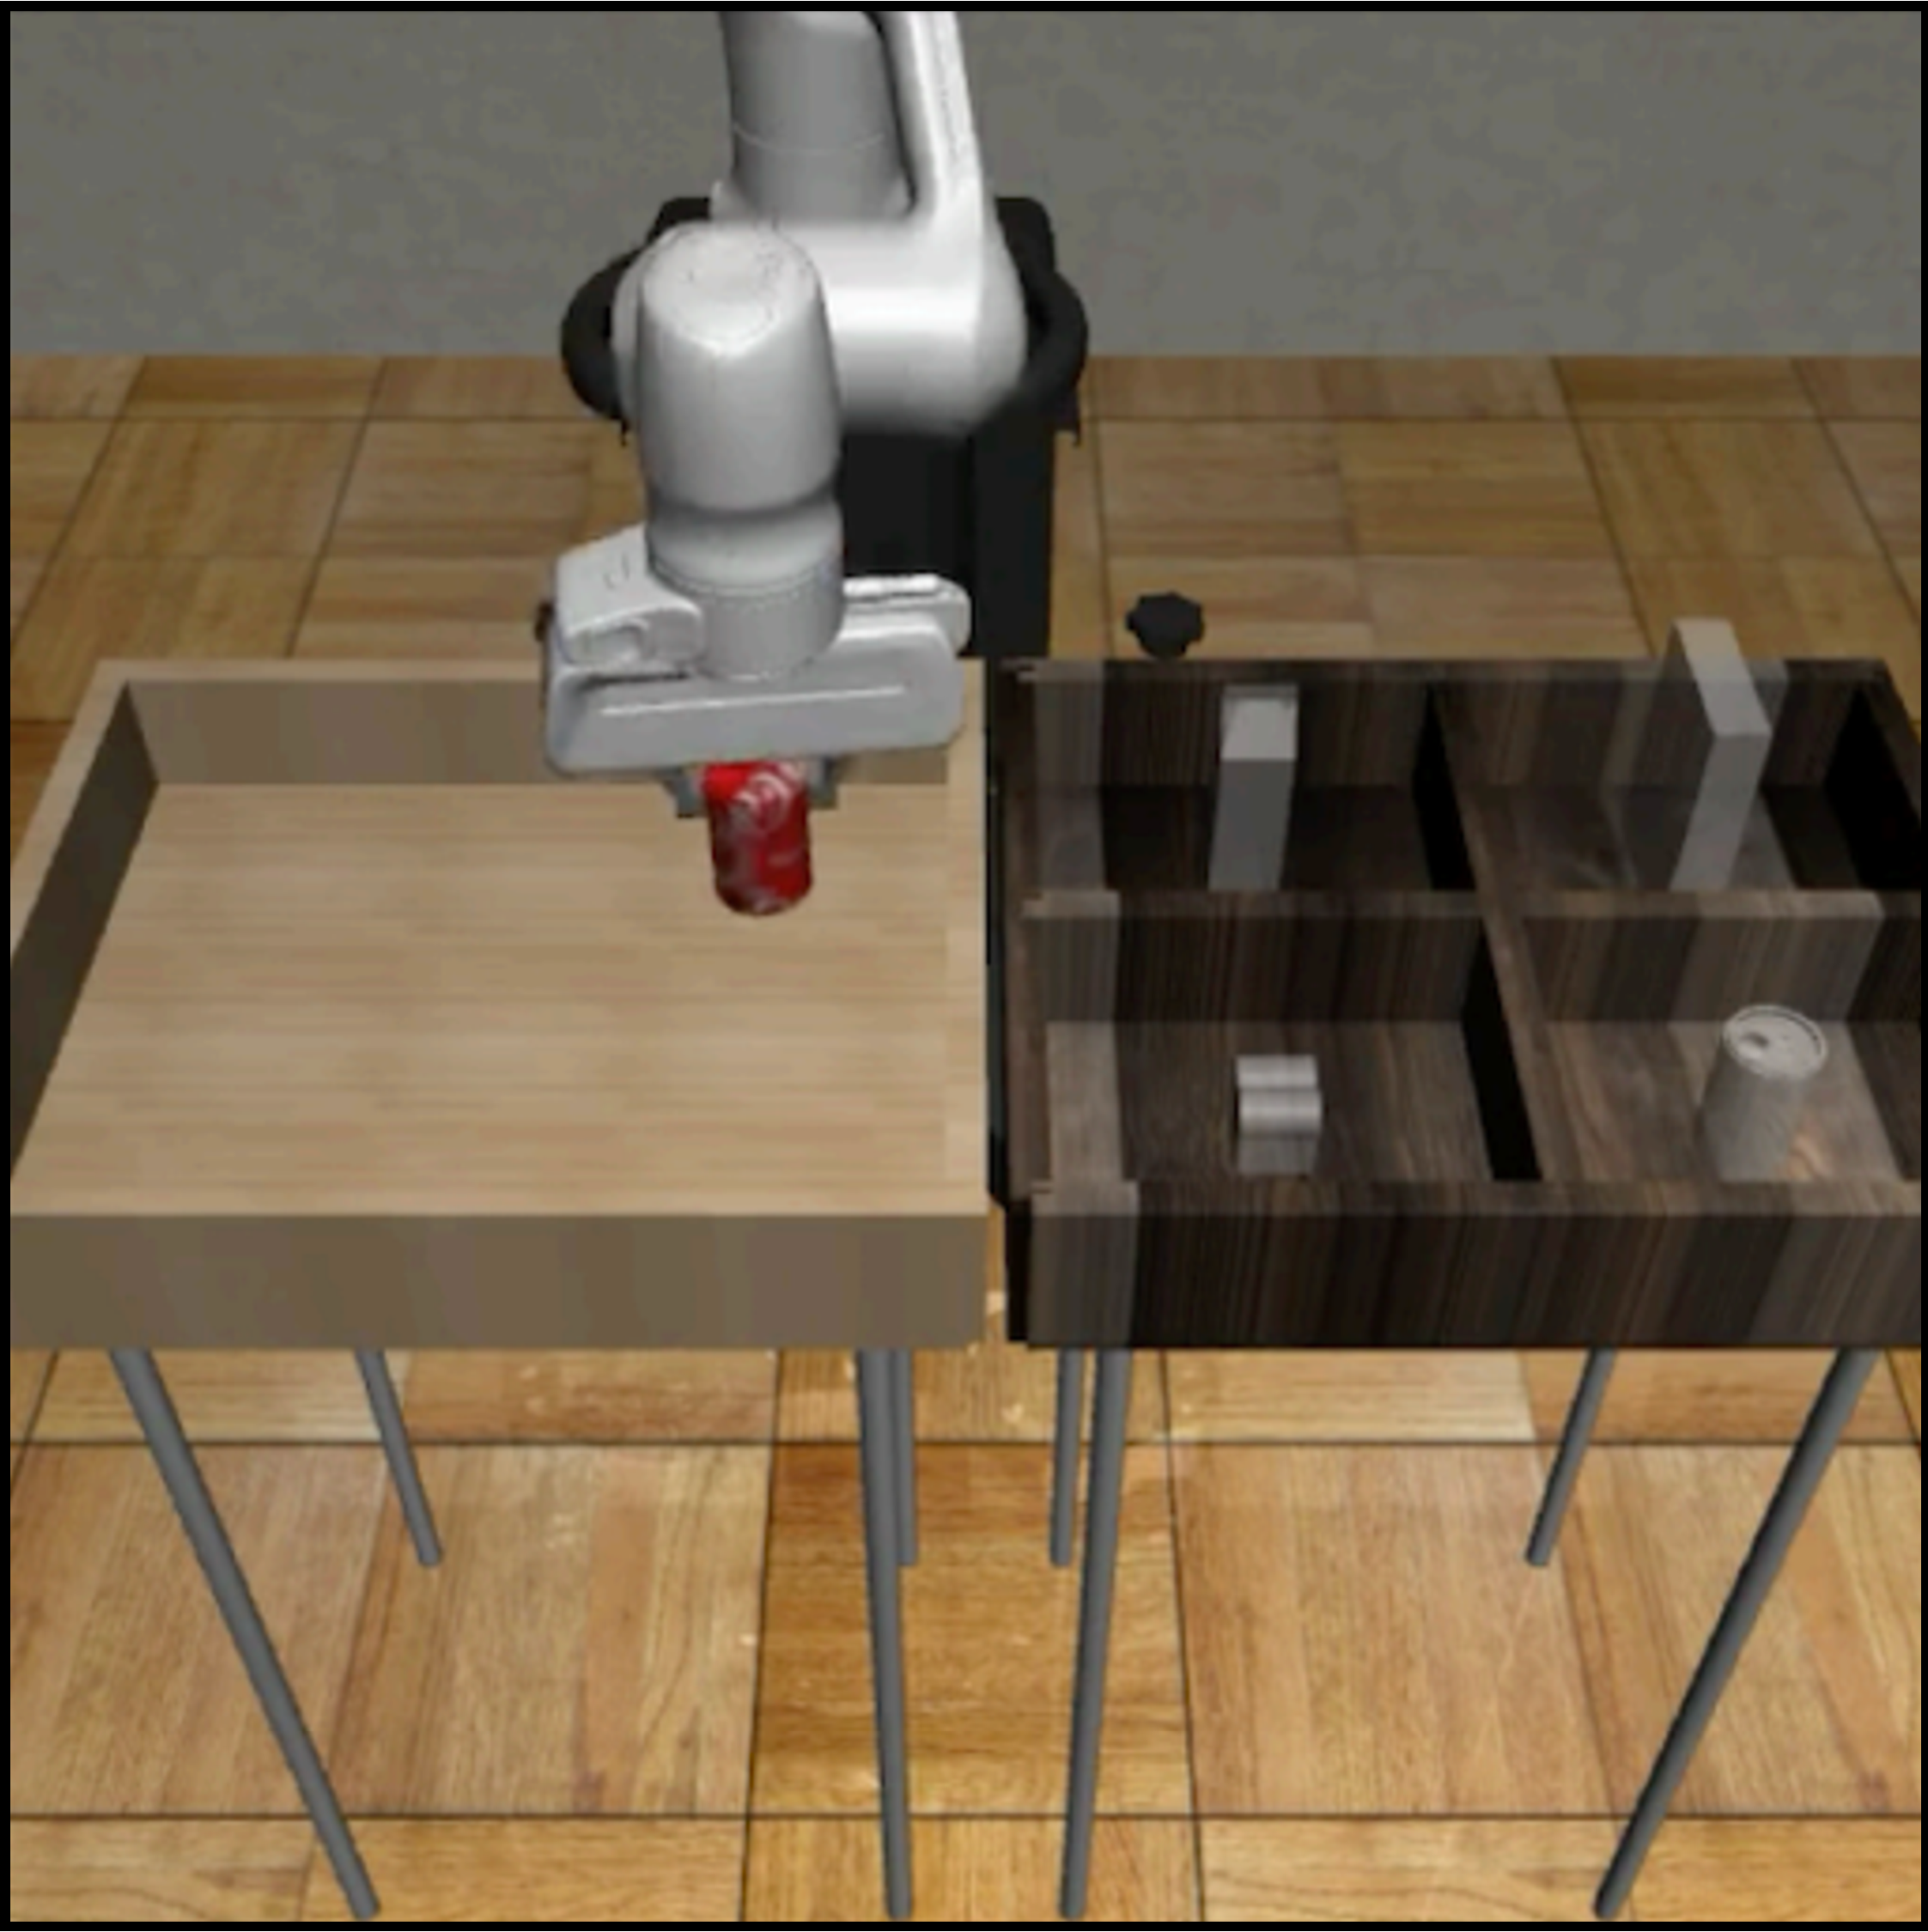
\includegraphics[width=\linewidth]{fig/tasks/can.pdf}
        \caption{Can}
        \label{fig:tasks:can}
    \end{subfigure} 
    \caption{
        We evaluate our method on five tasks that cover challenges such as exploration and planning over long horizons in RL settings, as well as object manipulation and continuous control in IL settings.
        Figures are from \citet{beattie2016deepmind} and \citet{mandlekar2021matters}.
    }
    \label{fig:tasks}
  \vspace{-1em}
\end{figure}

\para{Task-difficulty-based curriculum.} In the second instantiation, instead of taking snapshots of RL agents directly trained on test configurations, we collect learning progress on a series of easier but progressively harder tasks. For instance, in an embodied navigation task, the test configuration includes 20 rooms. Rather than logging source agents' learning progression in the 20-room maze, we record in a series of mazes with 5, 10, and 15 rooms. We then structure stored episodes first following learning progress and then the increase of layout complexity. This practice naturally creates a \textit{task-difficulty-based curriculum}, which resembles curriculum RL that is based on task difficulty ~\citep{matiisen2017teacherstudent,Narvekar2017AutonomousTS}.
We find it especially helpful for hard-exploration problems where the source RL agent does not make meaningful progress.

\para{Expertise-based curriculum.} For the setting of IL from mixed-quality demonstrations, we instantiate a curriculum based on demonstrators' expertise. This design choice is motivated by literature on learning from heterogeneous demonstrators~\citep{beliaev2022imitation, NEURIPS2021_670e8a43}, with the intuition that there is little to learn from novices but a lot from experts. To realize this idea, we leverage the Multi-Human dataset from RoboMimic~\citep{mandlekar2021matters}. Since it contains demonstrations collected by human demonstrators with varying proficiency, we organize offline demonstration trajectories following the increase of expertise to construct the \textit{expertise-based curriculum}.










